\chapter{Parâmetros de hélices e motores}
\label{sec:prop}
Todos os arquivos do simulador que iniciam com o prefixo \emph{prop} estão relacionados à descrição de um conjunto motor-hélice (atuadores do veículo). Sua estrutura principal pode ser verificada na figura \ref{fig:uml-01}.

\begin{figure}[!htb]
    \centering
    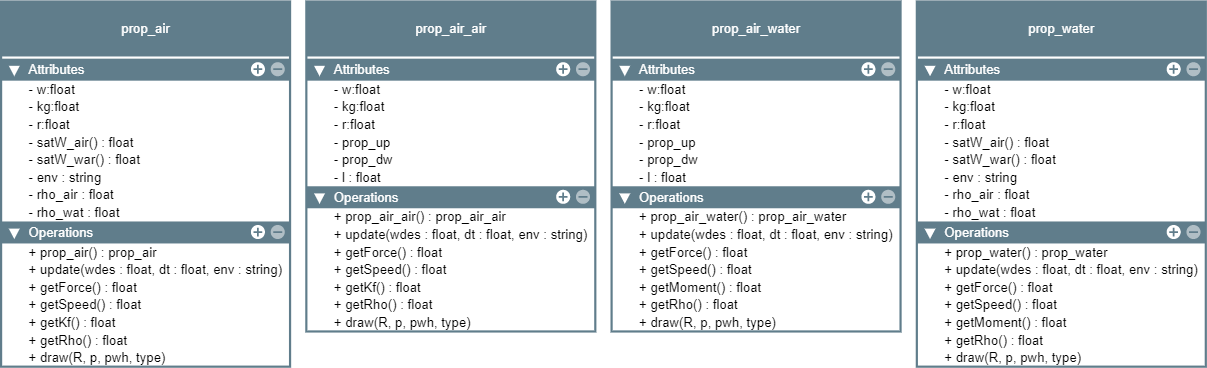
\includegraphics[width=\linewidth]{imagens/uml1.png}
    \caption{Diagrama UML das classes \emph{prop-}.}
    \label{fig:uml-01}
\end{figure}

\section{Classes \emph{prop\_air} e \emph{prop\_water}}
% utilizar \_ para evitar erros
As classes \emph{prop\_air} e \emph{prop\_water} são responsáveis por descrever dois tipos de conjuntos motor-hélice, respectivamente, aéreos e aquáticos. Estas são instanciadas nas classes \emph{prop\_air\_air} e \emph{prop\_air\_water}, nos objetos \emph{prop\_up} e \emph{prop\_dw}, os quais guardam a informação de qual tipo de conjunto é utilizado no ar e na água, respectivamente. Tal estrutura se deve à comparação de desempenho entre conjuntos aéreos e aquáticos para movimentação subaquática.

Conforme pode-se observar no trecho a seguir, a classe \emph{prop\_air}, bem como a classe \emph{prop\_water}, inicia com a declaração de algumas propriedades. Tais propriedades referem-se tanto a parâmetros específicos do conjunto motor-hélice, como, também, a propriedades relacionadas ao meio em que podem estar.

\lstinputlisting[language = Matlab, caption={propriedades da classe prop\_air},label={prop-air-1},firstnumber=3,linerange={3-17}]{codigos/prop_air.m}

Após a definição das propriedades das classes \emph{prop\_air} e \emph{prop\_water}, são criados os métodos das mesmas, os quais são responsáveis pela construção dos objetos, atualização das variáveis simuladas, retorno de valores para o código principal e pelo desenho das hélices na representação gráfica da simulação. O trecho a seguir mostra os métodos da classe \emph{prop\_air}.

\lstinputlisting[language = Matlab, caption={métodos da classe prop\_air},label={prop-air-1},firstnumber=19,linerange={19-91}]{codigos/prop_air.m}


\section{Classes \emph{prop\_air\_air} e \emph{prop\_air\_water}}
Os códigos para as classes \emph{prop\_air\_air} e \emph{prop\_air\_water} são similares entre si, diferindo apenas pela construção dos objetos. Para o primeiro, o atributo \emph{prop\_dw} recebe um objeto da classe \emph{prop\_air}, e para o segundo, o mesmo atributo recebe um objeto da classe \emph{prop\_water}.

Como esperado, as classes \emph{prop\_air\_air} e \emph{prop\_air\_water}, simplesmente agrupam os pares de atuadores, guardando as informações sobre cada um dos conjuntos motor-hélice. Assim, este código chama os métodos para os respectivos tipos de atuadores, conforme necessário.